\vspace{-1mm}
SHAP (SHapley Additive exPlanations) -- метод, оценивающий вклад признаков в предсказания модели на основе значений Шэпли.
\vspace{-3mm}

\subsubsection{Идея}
\vspace{-2mm}
Предсказание модели формируется на основе признаков. Если мы хотим узнать влияние отдельного признака, мы можем построить предсказание модели с ним и без него и затем посмотреть, как меняется результат. % почему реально не убирать насовсем?
Но модель может быть слишком сложной, чтобы мы могли оценить влияние предиктора по одному объекту, регулируя один признак при фиксированных остальных. Правильнее рассмотреть все возможные комбинации признаков: их разные значения, наличие/отсутствие, чтобы понять, как в каждом из перечисленных случаев добавление и исключение признака влияет на предсказание.

Рассматривая влияние признаков для разных объектов, мы получаем очень много предельных эффектов, что тяжело интерпретируется. Поэтому можно рассмотреть, какой в среднем эффект оказывает включение признака в модель. Тогда мы получим средневзвешенную оценку вклада отдельного предиктора в предсказание и сможем интерпретировать результат работы модели.
% Подумать, почему они сравнивают результат со средним кроме как кроме того что нужна всего одна модель и теряется точность

Однако для такого способа нужно либо обучить количество моделей, пропорциональное количеству всех комбинаций признаков -- которое растет экспоненциально с увеличением количества признаков. Либо оставлять пропущенные значения вместо исключенных признаков, что может плохо отразиться на качестве работы модели. Чтобы избежать этого, мы можем несколько видоизменить наше решение, не меняя цель. Вместо обучения дополнительной модели с меньшим количеством предикторов мы оценим ее предсказание, случайно изменяя исключенные признаки и усреднив результат.

Авторы алгоритма также вносят новую идею о способе расчета вклада признаков в предсказание: данные значения можно посчитать с помощью линейной регрессии с использованием матрицы весов определенного вида \cite{shap}.

\underline{Пример SHAP для табличных данных} \cite{shapgit}

\vspace{-4mm}
\begin{figure}[h]
	\centering{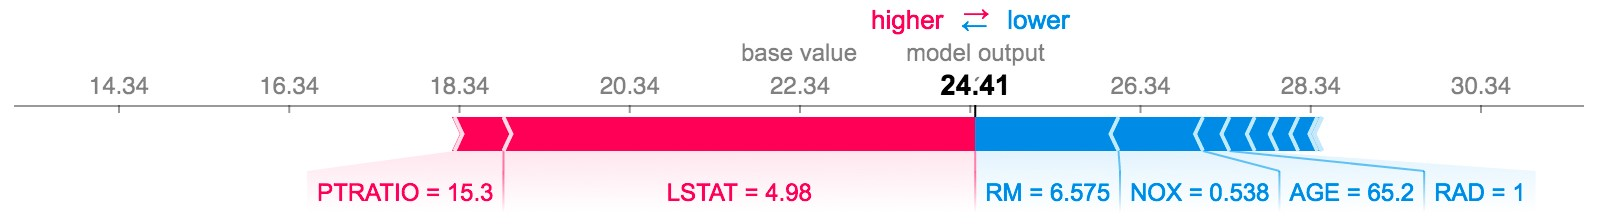
\includegraphics[width=\linewidth]{pics/shap1.png}}
\end{figure}
\vspace{-3mm}

В данном примере решалась задача регрессии, предсказание модели: 24.41. Отталкиваясь от base value как от исходного значения под воздействием влияния разных признаков (показаны стрелочками), данное наблюдение получило именно такой ответ, по мнению SHAP. Приведенные предикторы оказали наибольшее воздействие на результат работы модели. В аналогичном виде представляется интерпретация предсказаний для текстов.

\underline{Пример SHAP для картинок} \cite{shapgit}

\vspace{-2mm}
\begin{figure}[h]
	\centering{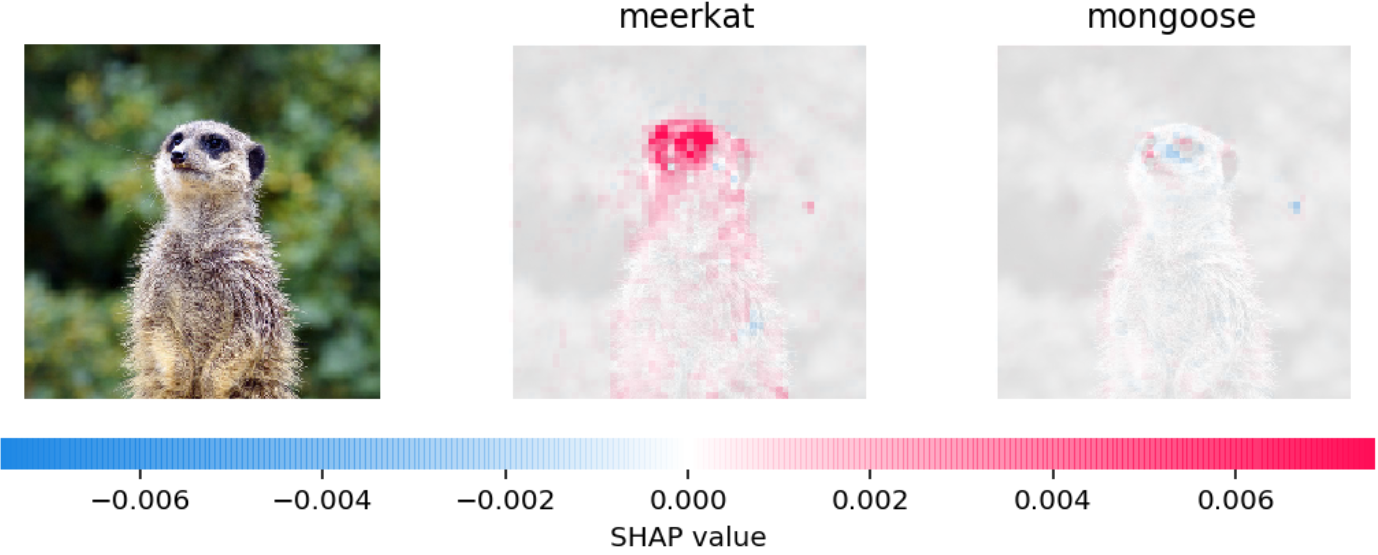
\includegraphics[width=0.65\linewidth]{pics/shap2.png}}
\end{figure}
\vspace{-2mm}

В данном случае SHAP, в отличие от LIME, работал с более мелкими признаками -- обычными пикселями. Значимость каждого признака показана с помощью цвета: чем насыщеннее цвет, тем сильнее он повлиял на результат. Красный цвет показывает положительное воздействие, синий цвет -- отрицательное. Однако SHAP может работать и с супер-пикселями, аналогично LIME.

\subsubsection{Значения Шэпли (Shapley values)}
Пусть $S$ -- множество не исключенных из модели признаков, в которое не входит исследуемый $i$-ый признак. Чтобы найти разницу предсказаний для признаков из $S$ и из $S \cup \{i\}$, куда входит $i$-ый признак, нам нужно обучить две модели, $f_S$ и $f_{S \cup \{i\}}$, соответственно. Тогда для объекта $x$ мы получим \cite{basis, shap}:
\[
f_{S \cup \{i\}}(x_{S \cup \{i\}}) - f_S(x_S),
\]
где $x_{S \cup \{i\}}$ -- объект $x$, у которого оставили только признаки из $S \cup \{i\}$, $x_S$ -- только признаки из $S$.

Как отмечалось ранее, значения данного выражения могут меняться при разных комбинациях признаков, поэтому мы усредним ее для всех возможных случаев. Считая, что $F$ -- множество всех признаков, получим итоговое выражение для $i$-го признака:
\vspace{-1mm}
\[
\phi_i = \frac{1}{|F|} \sum\limits_{S \subseteq F \backslash \{i\}}
\begin{pmatrix}
|F| - 1 \\
|S|
\end{pmatrix}^{-1}
(f_{S \cup \{i\}}(x_{S \cup \{i\}}) - f_S(x_S)),
\]
\vspace{-5mm}

где $|F|$ -- количество элементов в множестве $F$, $|S|$ -- в множестве $S$ \cite{basis, shap}.

Коэффициент:
\[
\ds \begin{pmatrix}
|F| - 1 \\
|S|
\end{pmatrix} = \frac{(|F|-1)!}{|S|! \cdot (|F| - |S| - 1)!}
\]
равен количеству всех возможных комбинаций признаков без учета исследуемого. Поделив на него, а также на количество признаков получаем среднее значение вклада признака.

Данный коэффициент также можно интерпретировать как вес комбинации при расчете среднего. Биномиальный коэффициент, равный количеству комбинаций, для одного или $|F|-1$ признаков меньше, чем для любого другого числа признаков. При делении на коэффициент мы получаем большее значение, который указывает на больший вес подобных комбинаций. Это имеет смысл, так как больше информации мы получаем, рассматривая влияние признаков по отдельности: либо оставляя только его, либо исключая все кроме него. С увеличением количества признаков в $S$ вес комбинации убывает.

Таким образом, мы получили величину, показывающую, какой в среднем вклад вносит конкретный признак в предсказание. Данное значение пришло из теории игр и носит название значение Шэпли (Shapley value). Они показывают, какой вклад внес в общий выигрыш отдельный игрок при кооперации. В нашей задаче мы рассматриваем предсказание модели как выигрыш, а признаки как игроков \cite{basis}.
\vspace{-2mm}